\begin{theorem}[O rozvoji holomorfní funkce na kruhu do mocninné řady]
Nechť $R \in (0, +\infty]$ a $f \in (U(z_0,R))$. Potom existuje jediná mocninná řada $\sum\limits _{n=0} ^{\infty} a_n(z-z_0)^n$, která má na $U(z_0,R)$ součet $f$. Navíc platí, že $a_n=\frac{f^{(n)}(z_0)}{n!}$, $n \in \mathbb{N}_0$.
\end{theorem}

\begin{proof}
\begin{enumerate}
    \item jednoznačnost: Zřejmě z toho, že $a_n=\frac{f^{(n)}(z_0)}{n!}$, $n \in \mathbb{N}_0$.
    \item existence: Nechť $z \in U(z_0, R)$. Volme $r>0$, aby $|z-z_0|<r<R$. Potom z (CV$_z$) je (1) $f(z)=\frac{1}{2 \pi i} \int_\varphi \frac{f(w)}{w-z} \diff w$, kde $\varphi(t)=z_0+re^{it} \text{, } t \in [0, 2\pi]$.
    
    Pro každé $w \in \langle \varphi \rangle$ máme
    
    $$(2) \quad \frac{1}{w-z}=\frac{1}{(w-z_0)-(z-z_0)}=\frac{1}{w-z_0}\cdot\frac{1}{1-\frac{z-z_0}{w-z_0}}=\sum_{n=0}^\infty \frac{(z-z_0)^n}{(w-z_0)^{n+1}} \text{.}$$
    Kde $|\frac{z-z_0}{w-z_0}|=1$ a suma konverguje stejnoměrně pro $w \in  \langle \varphi \rangle$. Dosadíme (2) do (1). Potom
    \begin{equation*}
        \begin{split}
    f(z) &=\frac{1}{2 \pi i} \int_\varphi \sum_{n=0}^\infty \frac{(z-z_0)^n}{(w-z_0)^{n+1}} f(w) \diff w= 
    \sum_{n=0}^\infty (z-z_0)^n \frac{1}{2 \pi i} \int_\varphi \frac{f(w)}{(w-z_0)^{n+1}} \diff w \\
     &=\sum_{n=0}^\infty (z-z_0)^n \frac{f^{(n)}(z_0)}{n!} \text{ z (CV}_z^{(n)} \text{).}
     \end{split}
    \end{equation*}
\end{enumerate}
\end{proof}

\begin{example}
$e^z=\sum\limits_{n=0}^\infty \frac{z^n}{n!}$, $z \in \mathbb{C}$, protože $\exp \in \mathcal{H}(\mathbb{C})$ a $\exp^{(n)}(0)=\exp(0)=1$.
\end{example}

\begin{theorem}[O nulovém bodě]
Nechť $f$ je holomorfní funkce na okolí $z_0 \in \mathbb{C}$ a $f(z_0)=0$. Potom buď
\begin{enumerate}
    \item existuje $r>0$, že $f=0$ na $U(z_0,r)$, anebo
    \item existuje $r>0$, že $f\neq 0$ na $P(z_0,r):=U(z_0,r)\backslash \{z_0\}$.
\end{enumerate}
V případě 2. existuje jediné $p\in \mathbb{N}$ takové, že (0) $f(z_0)=f'(z_0)= \ldots = f^{(p-1)}(z_0)=0$, $f{(p)}(z_0) \neq 0$. Číslo $p$ nazýváme násobnost nulového bodu $z_0$ funkce $f$.
\end{theorem}

\begin{note}
Navíc $z_0$ je nulový bod $f$ násobnosti $p$, právě když existuje $r>0$ a $g \in \mathcal{H}(U(z_0,r))$ tak, že $\forall z \in U(z_0,r)$: ($\triangle$) $g(z) \neq 0$ a $f(z)=(z-z_0)^pg(z)$.
\end{note}

\begin{proof}
Máme, že $f(z)=\sum\limits _{n=0} ^{\infty} a_n(z-z_0)^n$, $z \in U(z_0,r)$. Pokud nenastane 1., potom existuje $n \in \mathbb{N}$, že $0 \neq a_n=\frac{f^{(n)}(z_0)}{n!}$. Zvolme nejmenší $p \in \mathbb{N}$, aby $a_p \neq 0$. Potom platí (0) a $\forall z \in U(z_0,r)$: $f(z)=a_p(z-z_0)^p + \ldots = (z-z_0)^p \cdot \sum\limits_{n=p}^\infty a_n(z-z_0)^{n-p}$. Dále $g(z)$ definujeme jako poslední sumu.%Nebo-li g(z):=\sum\limits_{n=p}^\infty a_n(z-z_0)^{n-p}$
Protože $g(z_0)=a_p \neq 0$, existuje $r>0$, že $g \neq 0$ na $U(z_0,r)$ a $f(z)=(z-z_0)^pg(z) \neq 0$ na $P(z_0,r)$. Obrácené tvrzení plyne snadno.
\end{proof}

\begin{theorem}[O jednoznačnosti pro holomorfní funkce]
Nechť $\emptyset \neq G \subset \mathbb{C}$ je oblast a $f,g \in \mathcal{H}(G)$. Pak jsou následující tvrzení ekvivalentní:
\begin{enumerate}
\item $f=g$ na $G$;
\item množina $M:=\{z \in G | f(z)=g(z) \}$ má v $G$ hromadný bod, tj. existuje $z_0 \in G$ takový, že $M \cap P(z_0,r) \neq \emptyset  \; \forall  r>0$;
\item existuje $z_0 \in G$, že $f^{(k)}(z_0)=g^{(k)}(z_0) \; \forall k \in \mathbb{N}_0$.
\end{enumerate}
\end{theorem}

\begin{proof}
BÚNO $g \equiv 0$ na $G$ (jinak uvažme $f-g$).

1 $\Rightarrow$ 2, 2 $\Rightarrow$ 3 Nechť $z_0 \in G$ je hromadný bod $M:=\{z \in G | f(z)=0 \}$. Z věty o nulovém bodě je $f=0$ na nějakém okolí $z_0$, tudíž platí 3.

3 $\Rightarrow$ 1 Nechť $N:=\{z \in G | \forall k \in \mathbb{N}_0: f^{(k)}(z_0)=0 \}$. Potom $\emptyset  \neq N$, $N$ je uzavřená v $G$, protože všechny $f^{(k)}$ jsou spojité. Navíc $N$ je otevřená. Nechť $z_1 \in \mathbb{N}$. Podle věty o nulovém bodě existuje $r>0$, že $f=0$ na $U(z_1,r)$. Tedy $U(z_1,r) \subset N$. Protože $G$ je oblast, dostaneme $N=G$ a speciálně 1.
\end{proof}

\begin{example}
Vzoreček $\sin (2z)=2\sin (z) \cos (z)$, $z \in \mathbb{C}$ dostaneme z věty o jednoznačnosti, protože obě strany rovnosti jsou celé funkce a víme, že rovnost platí na $\mathbb{R}$ (tzn. platí 2).
\end{example}

\begin{note}
Podobně lze řadu vzorečků bez počítání zobecnit z $\mathbb{R}$ do $\mathbb{C}$!
\end{note}

\begin{theorem}[Princip maxima modulu]
Nechť $G \subset \mathbb{C}$ je oblast a $f\in \mathcal{H}(G)$. Potom je $f$ konstantní na $G$, pokud $|f|$ nabývá na $G$ lokální maximum, tzn. existuje $z_0 \in G$ a $r>0$ tak, že $\forall z \in U(z_0,r) \subset G: |f(z)| \leq |f(z_0)|$. (+)
\end{theorem}

\begin{proof}
Nechť platí (+). Potom $f(z)=\sum\limits_{n=0}^\infty a_n(z-z_0)^{n}$, $z\in U(z_0,r)$. Pro $0<\rho<r$ platí, že $|a_0|^2=|f(z_0)|^2\geq \frac{1}{2 \pi} \int_{0}^{2 \pi} |f(z_0+\rho e^{it})|^2 \diff t=%tato rovnost plyne z toho,že $|f(z)|^2=f(z)\cdot \overline {f(z)}$
\frac{1}{2 \pi} \int_{0}^{2 \pi} (\sum\limits_{n=0}^\infty a_n \rho^n e^{int})(\sum\limits_{m=0}^\infty \overline{a_m} \rho^m e^{-imt}) \diff t=%Jelikož obě řady konvergují stejnoměrně a absolutně pro $t\in[0,2\pi]$, tak i jejich součin konverguje stejnoměrně a absolutně.
\sum\limits_{n=0}^\infty \sum\limits_{m=0}^\infty a_n\ \cdot \overline{a_m} \rho^{n+m} \frac{1}{2 \pi} \int_{0}^{2 \pi}  e^{it(n-m)} \diff t=\sum\limits_{n=0}^\infty |a_n|^2\rho^{2n}$, nebot $\frac{1}{2 \pi} \int_{0}^{2 \pi}  e^{it(n-m)} \diff t=0$, pro $n\neq m$ a \newline $\frac{1}{2 \pi} \int_{0}^{2 \pi}  e^{it(n-m)} \diff t=1$, pro $n=m$.
Nebo-li $|a_0|^2\geq|a_0|^2+|a_1|^2\rho^2+\cdots$, tudíž $0=a_1=a_2=\cdots$. Dostáváme,že $f=a_0$ na $U(z_0,r)$ a z věty o jednoznačnosti $f=a_0$ na $G$.
\end{proof}

\section{\texorpdfstring{Riemannova sféra}{Riemannova sféra}}
Rozšíříme $\mathbb{C}$ o \emph{nekonečno}.
Položíme $\$=\mathbb{C}\cup\{\infty\}$, kde $\infty\notin\mathbb{C}$, a zavedeme \emph{okolí} kolem $\infty$
$P(\infty,\varepsilon):=\{z\in\mathbb{C}\mid |z|>\frac{1}{\varepsilon}$, $\varepsilon>0$,
$U(\infty,\varepsilon):=P(\infty,\varepsilon)\cup \{\infty\}$.

\begin{definition}
Řekneme, že $z_n\rightarrow z_0$ v $\$$, pokud $\forall\varepsilon>0\textbf{ }  \exists n_0\in\mathbb{N}\textbf{ }\forall n\geq n_0:z_n\in U(z_0,\varepsilon)$.
\end{definition}

\begin{note} Z definice plyne:
\begin{itemize}
    \item $z_n\rightarrow z_0$ v $\$$ a $z_0\in\mathbb{C}\Leftrightarrow z_n\rightarrow z_0$ v $\mathbb{C}$.
    \item $z_n\rightarrow\infty\Leftrightarrow|z_n|\rightarrow+\infty\Leftrightarrow\frac{1}{z_n}\rightarrow\cdot$. Zde $\frac{1}{\infty}:=0$ a $|\infty|:=+\infty$.
\end{itemize}
\end{note}

\begin{note}
$\$$ je jednobodová kompaktifikace topologického prostoru $\mathbb{C}$.
\end{note}

\begin{properties}%proč se Riemannově sféře říká Riemannova sféra
Na $\$$ zavedeme metriku $\rho$ (není jediná), tž.
(*)$z_n\rightarrow z_0$ v $\$\Leftrightarrow \rho(z_n,z_0)\rightarrow 0$. Navíc $(\$,\rho)$ bude \emph{izometrický} s jednotkovou sférou $S^2:=\{(\alpha,\beta,\gamma)\in\mathbb{R}^3\mid \alpha^2+\beta^2+\gamma^2=1\}$, kterou chápeme jako metrický podprostor $\mathbb{R}^3$. Speciálně $(\$,\rho)$ je \emph{kompaktní}.
\begin{itemize}
    \item Definujeme \emph{stereografickou projekci} $\phi:\mathbb{C}\rightarrow S^2\smallsetminus \{N\}$ jako na obrázku, kde $N=(0,0,1)$.
    $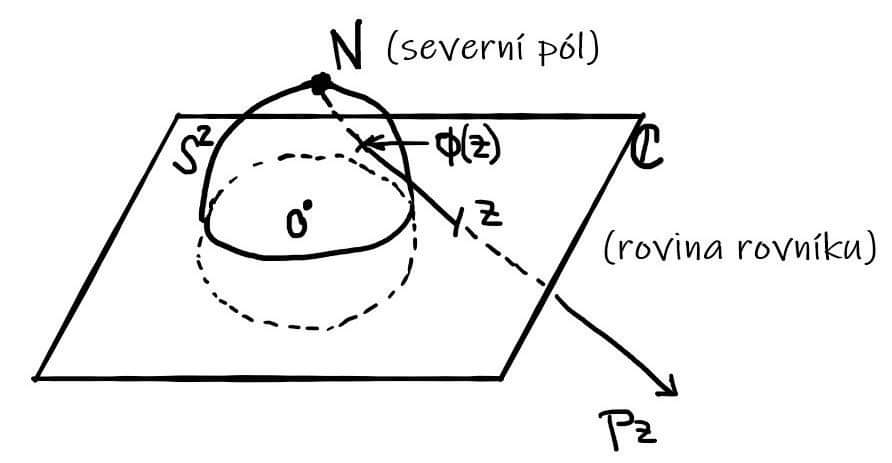
\includegraphics[width=\textwidth]{images/obrazek1.jpeg}$ 
    Položme $\phi(\infty):=N$. Pro $z\in\mathbb{C}$ je $\{\phi(z)\}=(S\smallsetminus \{N\})\cap p_z$, kde $p_z$ je polopřímka z $N$ procházející bodem $z\in\mathbb{C}$. Potom $\phi:\$\xrightarrow[]{na}S^2$ je bijekce.
    \begin{excercise}(CV) 
     \begin{itemize}
        \item $\phi(z):=(\frac{2x}{x^2+y^2+1},\frac{2y}{x^2+y^2+1},\frac{x^2+y^2-1}{x^2+y^2+1})$, $z=x+iy \in \mathbb{C}$.
        \item $\phi^{-1}(\alpha,\beta,\gamma):=(\frac{\alpha}{1-\gamma},\frac{\beta}{1-\gamma})$, $(\alpha,\beta,\gamma)\in S^2\smallsetminus \{N\}$
     \end{itemize}
    \end{excercise}
    \item Položme $\rho(\cancel{z},w):=|\phi(z)-\phi(w)|$, $z,w\in\$$, kde $|\cdot|_S$ je Eukleidovská norma  v $\mathbb{R}^3$.($\phi$ je izometrie $(\cancel{\$},\rho)$ na $S^2$)
     
    \item Platí (*). Skutečně z předchozího bodu a z cvičení máme: $\rho(z_n,z_0)\rightarrow0\Leftrightarrow\phi(\cancel{z_n}\rightarrow\phi(\cancel{z_0})\Leftrightarrow z_n\rightarrow \cancel{z_0} v \cancel{\$}$, protože $\phi$ i $\phi^{-1}$ jsou spojité.
    \end{itemize}
     \begin{example}
     Necht $z_n\in \mathbb{C}$ a $z_n\rightarrow \infty$. Potom $|z_n|\rightarrow+\infty\Rightarrow \phi(z_n)\in S^2; \phi_3(z_n)\rightarrow 1 \Rightarrow \phi(z_n)\rightarrow N:=(0,0,1)$
     \end{example}
     \begin{example}
     Necht $(\alpha,\beta,\gamma)\in S^2\smallsetminus\{N\}$ a $(\alpha,\beta,\gamma)\rightarrow N$. Potom
     $|\phi^{-1}(\alpha_n,\beta_n,\gamma_n)|^2=\frac{1-\gamma_n^2}{(1-\gamma_n)^2}=\frac{1+\gamma_n}{1-\gamma_n}\rightarrow+\infty\Rightarrow\phi^{-1}(\alpha_n,\beta_n,\gamma_n)\rightarrow\infty$
     
     \end{example}

\end{properties}
